\chapter{Optimizing patients travel}

\section{Context}

Cancer treatment delay is a problem in health systems worldwide, increasing mortality for many types of cancers \cite{hanna_mortality_2020}, including breast cancer \cite{caplan_delay_1992, williams_assessment_2015, pace_delays_2015}. Distance between patients residence and diagnosing hospitals is among the factors causing these delays, especially for cancer types that are hard to diagnose \cite{flytkjaer_virgilsen_cancer_2019}. While accessibility to healthcare is growing, research found that 8.9\% of the global population (646 million people) could not reach healthcare within one hour if they had access to motorized transport \cite{weiss_global_2020}. Thus, a non insignificant part of the population might be exposed to lower prognosis.

\subsection{Centralized care}

Northern countries, such as the UK, USA and Canada, have been implementing a policy of centralizing the care of patients for many specialized services \cite{kelly_are_2016}. With such policy, patients are directed to a limited number of hospitals with higher volumes and more specialized surgeons. Centralized care is beneficial for patients undergoing high-risk procedures, these surgeries have lower mortality rates when performed by high-volume surgeons \cite{pekala_centralization_2021,birkmeyer_surgeon_2003,finks_trends_2011,hollenbeck_getting_2007,goossens-laan_systematic_2011}.

However, the benefits of centralized healthcare have been debated. A centralized approach often requires patients to travel far away from their home and their local community hospitals \cite{woo_centralisation_2012}. Patients subject to longer travels to reach a specialized hospital are likely to be affected by the travel burden and separation from their social environment \cite{payne_impact_2000}. In the debate between local versus centralized healthcare provision, there are evidence of an association between travel distance and health outcomes \cite{kelly_are_2016}.

\subsection{The impact of travelling on cancer patients}

We are now interested in the impact of travel on cancer patients. Unsurprisingly, travel to cancer treatment is inconvenient for some patients and might even act as a barrier to treatment \cite{payne_impact_2000}. Research also showed that patients who lived far from hospitals and had to travel more than 50 miles had a more advanced stage at diagnosis, lower adherence to encoded treatments, a worse prognosis, and a worse quality of life \cite{ambroggi_distance_2015}. More research linked travel burden with lower treatment compliance \cite{dutta_evaluation_2013,guidry_transportation_1997}. The distance from the hospital influences the choice of appropriate treatment by cancer patients. In breast cancer, patients living farther from a radiation treatment facility more often underwent mastectomy instead of breast conservative surgery \cite{schroen_impact_2005,celaya_travel_2006,voti_treatment_2006,meden_relationship_2002,nattinger_relationship_2001,boscoe_geographic_2011} or did not undergo radiotherapy after breast cancer surgery \cite{satasivam_dilemma_2014,schroen_impact_2005,celaya_travel_2006}. In non small cell lung cancer, patients were most likely to not undergo potentially curative surgery if they lived far from a specialist hospital and only attended a general hospital for their care \cite{tracey_patients_2015}. Moreover, the necessity for repeated visits for cancer diagnosis and treatment makes distance an even more important issue for the patient\cite{guidry_transportation_1997}. However, for hard to diagnose cancer type like rectum or testis cancers, distance was associated with decreasing odds of advanced disease stage \cite{virgilsen_travel_2019}. This is possibly due to being treated in more specialized hospitals.

\subsection{Living in rural areas}

The negative effects of centralized healthcare are even more pronounced for patients living in rural areas. Indeed, rural cancer patients face more challenges in receiving care, due to the limited availability of providers and clinical trials, as well as transportation barriers and financial issues \cite{charlton_challenges_2015}. There are evidence of poorer treatments and outcomes for patients living in rural areas. For instance, in Australia, poorer survival and variations in clinical management have been reported for breast cancer women living in non metropolitan areas \cite{dasgupta_variations_2018}. Still in Australia, breast cancer women treated in a rural hospital had a reduced likelihood of breast conservative surgery \cite{hall_unequal_2004}.  The hazard of death from ovarian cancer was greater in women treated at a public general hospital than in women treated at a gynecological oncology service (GOS) \cite{tracey_effects_2014}. Contacting a provincial hospital instead of a university hospital might lead to diagnosis and treatment delays, which could be improved by a better referral system \cite{thongsuksai_delay_2000}. In Australia, patients living farther from a radiotherapy service were more likely to die of rectal cancer, with a 6\% risk increase for each additional 100km \cite{baade_distance_2011}. In Rwanda, rural breast cancer patients who lived in the same district as breast cancer hospitals had a decreased likelihood of system delay \cite{pace_delays_2015}. In Canada, place of residence seems to influence health outcomes in patients with diffuse large B-cell lymphoma \cite{lee_effect_2014}. They found that rural and metropolitan patients had similar survival; however, patients in small and medium urban areas experienced worse outcomes than those in metropolitan areas. Thus, rural culture might have a dual effect on health outcomes. On one hand, distance, transportation, and health services shortage are barriers to healthcare. On the other hand, rural culture comes with community belonging, and deeper relationship with health care professionals, which might be beneficial for some patients \cite{brundisini_chronic_2013}.

\subsection{Health and climate change}

The World Health Organization called climate change the greatest threat to global health in the 21st century, significantly affecting hundreds of millions of people \cite{change_climate_2015}. The United Nations created the \ac{ipcc} to assess the science related to climate change and provide governments with scientific information that they can use to develop climate policies.
The health care sector is an important contributor to \ac{co2} emissions. An international comparison of health care carbon footprints showed that, on average, the health carbon footprint in 2014 constituted 5.5\% of the total national carbon footprint \cite{pichler_international_2019}. Hence, the health sector has a responsibility to take climate action \cite{health_care_without_harm_hcwh_global_2021}. Especially since the Paris Agreement, where countries agreed to cut \ac{ghg} emissions to keep global warming below 2°C. Today, hospitals are powered by fossile energy such as coal, oil and gas. Healthcare related travels, and the manufacture and transport of healthcare products are also major causes of \ac{ghg} emissions. Ultimately, all health systems will need to reach near zero emissions by 2050, which can be more cost effective than business as usual. The Lancet Countdown on health and climate change started to review annually the relation between health and climate change \cite{watts_2020_2021}. A large share of these carbon emissions is due to patients journeys \cite{andrews_carbon_2013,nicolet_what_2022} because most patients travel by car \cite{forner_carbon_2021}. With centralization of care, patients are encouraged to be treated in large hospitals for better outcome \cite{eskander_health_2016}. Such hospitals are in urban areas, and the populations living in rural areas will have to travel longer to reach these centers, resulting in higher carbon emissions.

In France, few studies have evaluated the ecological impact of cancer care \cite{guillon_empreinte_2020}. The Shift Project is a French think tank that works towards a carbon-free economy. As a non-profit organization, they inform and influence the debate on the energy transition. In 2021, the Shift Project released a report on how to decarbonize the health care sector in France \cite{the_shift_project_plan_2021}. They identified that most of the \ac{ghg} emissions were scope 3 emissions, which are indirect emissions that occur in the hospitals value chain. Among these emissions, the largest source are pharmaceuticals and medical device buying, followed by patients and visitors transportation. The Shift Project states that emissions related to transportation should be cut by 99\%, through measures like increasing public transportation and telemedicine.

\subsection{Telemedicine}

Teleoncology models are used increasingly throughout the world as a means to provide access to quality cancer care for people in rural, remote and other disadvantaged settings. Some authors have suggested that teleoncology is merely about avoiding long distance travel. In this commentary we argue that the benefits of teleoncology extend beyond those of the patients and their families to the rural health system and beyond \cite{sabesan_are_2014}.

Teleoncology model of care allows rural and Indigenous cancer patients to receive specialist consultations and chemotherapy treatments closer to home, thus minimising the access difficulties faced by the rural sector \cite{sabesan_telemedicine_2012}.

It is feasible for medical oncologists from tertiary centres to assess acute cancer patients and initiate cancer care in a timely and safe fashion at rural hospitals through the use of telemedicine, if the infrastructure and human resources are adequate at the rural sites \cite{sabesan_timely_2014}.

While most centers use teleoncology to complement their face-to-face outreach services, some centers have replaced face-to-face with teleoncology models. This was accepted by the patient after explaining to them why a physical examination was not always required. Patients had a physical exam within 60 days of their telehealth consultation. Importantly, there were no changes in the clinical management due to the lack of physical examination by specialists. Telesupervision models can be beneficial in training medical, nursing, and allied health trainees and staff at rural centers \cite{sabesan_medical_2014}.

Our evaluation suggests that teleoncology is an acceptable model of care for Indigenous patients, with high levels of satisfaction expressed from patients, families and HWs. Strategies for change are: Mandatory informed consent procedure for all patients offered with VC; Formalised competency training for staff in skills essential to maintain safe practices in teleoncology; Clear clinical documentation to facilitate improved communication in patient management between medical staff at main centre and distant sites; Further efforts in promotion, education and support for staff to participate in telemedicine \cite{mooi_teleoncology_2012}.

Describe the different e-health tools and their potential clinical impacts in oncology, as already reported at every level of care, including education, prevention, diagnosis, treatment, and monitoring \cite{bertucci_outpatient_2019}:

\begin{enumerate}
    \item Education: From the patient perspective, the lack of general information on diseases and treatments is a major issue concerning participation in the decision-making for and adherence to treatments. Websites, social networks, forums, and smartphone applications could solve this issue as they enable immediate access to unlimited information. Access to information is also important for oncologists in routine practice, and these allow for rapid access to the most recent and up-to-date data, guidelines, drug lists, and corresponding toxicities.
    \item Prevention: Websites inform patients about potential risk factors and also help with modifying exposure. Smartphone applications can repeatedly deliver proactive and discreet information and advice anywhere and at any time, immediately attracting the user's attention and prompting for urgent responses as necessary according to the context.
    \item Screening: Screening may also be improved by e-health [50], notably for cervical cancer. In Tanzania, a screening program dedicated to cervical uterine carcinoma was set up using smartphones. Nurses located in the most distant regions of the country used their smartphones to take pictures of cervices and send them by multimedia messaging service (MMS)to physicians in a cancer center. The physicians would then respond via text message with the appropriate actions to take.
    \item Diagnosis: Diagnosis may also benefit from e-health tools that allow for remote clinical examination, as recently reported for non-invasive detection of anemia using only patient-sourced photos.
    \item Treatment: E-health could be a major asset in facilitating treatment ``outside the walls'', by aiding in improved compliance, toxicity management, and earlier discharge from hospitals.
    \item Post-Treatment Follow-Up: Follow-up consultations aim for the early detection of relapses and management of possible persistent or late drug toxicities, and also identify disease-related psychological, social, and professional problems in patients' and families' lives. Unfortunately, general practitioners feel poorly trained in these areas while patients prefer trusting their oncologist. However, for oncologists, the average duration for consultations has not changed, even though the number of consultations is constantly increasing. Access to these consultations in cancer centers may also be problematic for patients that live far from the hospital or have transportation difficulties, which likely contributes to the relatively worse outcomes of patients living in rural areas or underserved suburbs. E-health could solve these issues as well via virtual consultations with oncologists. Digital follow-up may also improve survival. E-health technologies may also improve the quality of survival. They promote emotional well-being in breast cancer patients within the three months of diagnosis.
\end{enumerate}

% Telemedicine limitations
Cancer care ``outside the walls'' is becoming a critical issue and will have human, economic, and organizational consequences. Besides the expected benefits, several questions and fears are emerging \cite{bertucci_outpatient_2019}. However, evaluation of mobile applications is crucial and several studies have pointed out significant drawbacks, such as a lack of updates and medical scientific validation. There are also questions regarding the risk of patient morale and isolation. Another important challenge is the need for physical examination, as it is more difficult to build an atmosphere of trust during remote consultations and the examinations are of inferior quality. A further potential limitation of e-health is the digital divide, i.e., certain categories of patients (elderly, fragile, foreign, poorly educated, rural, etc.) have difficulties in accessing the Internet or do not have the necessary broadband connections.

\section{Methods}
% TODO

\section{Results}
% TODO

\begin{figure}[H]
    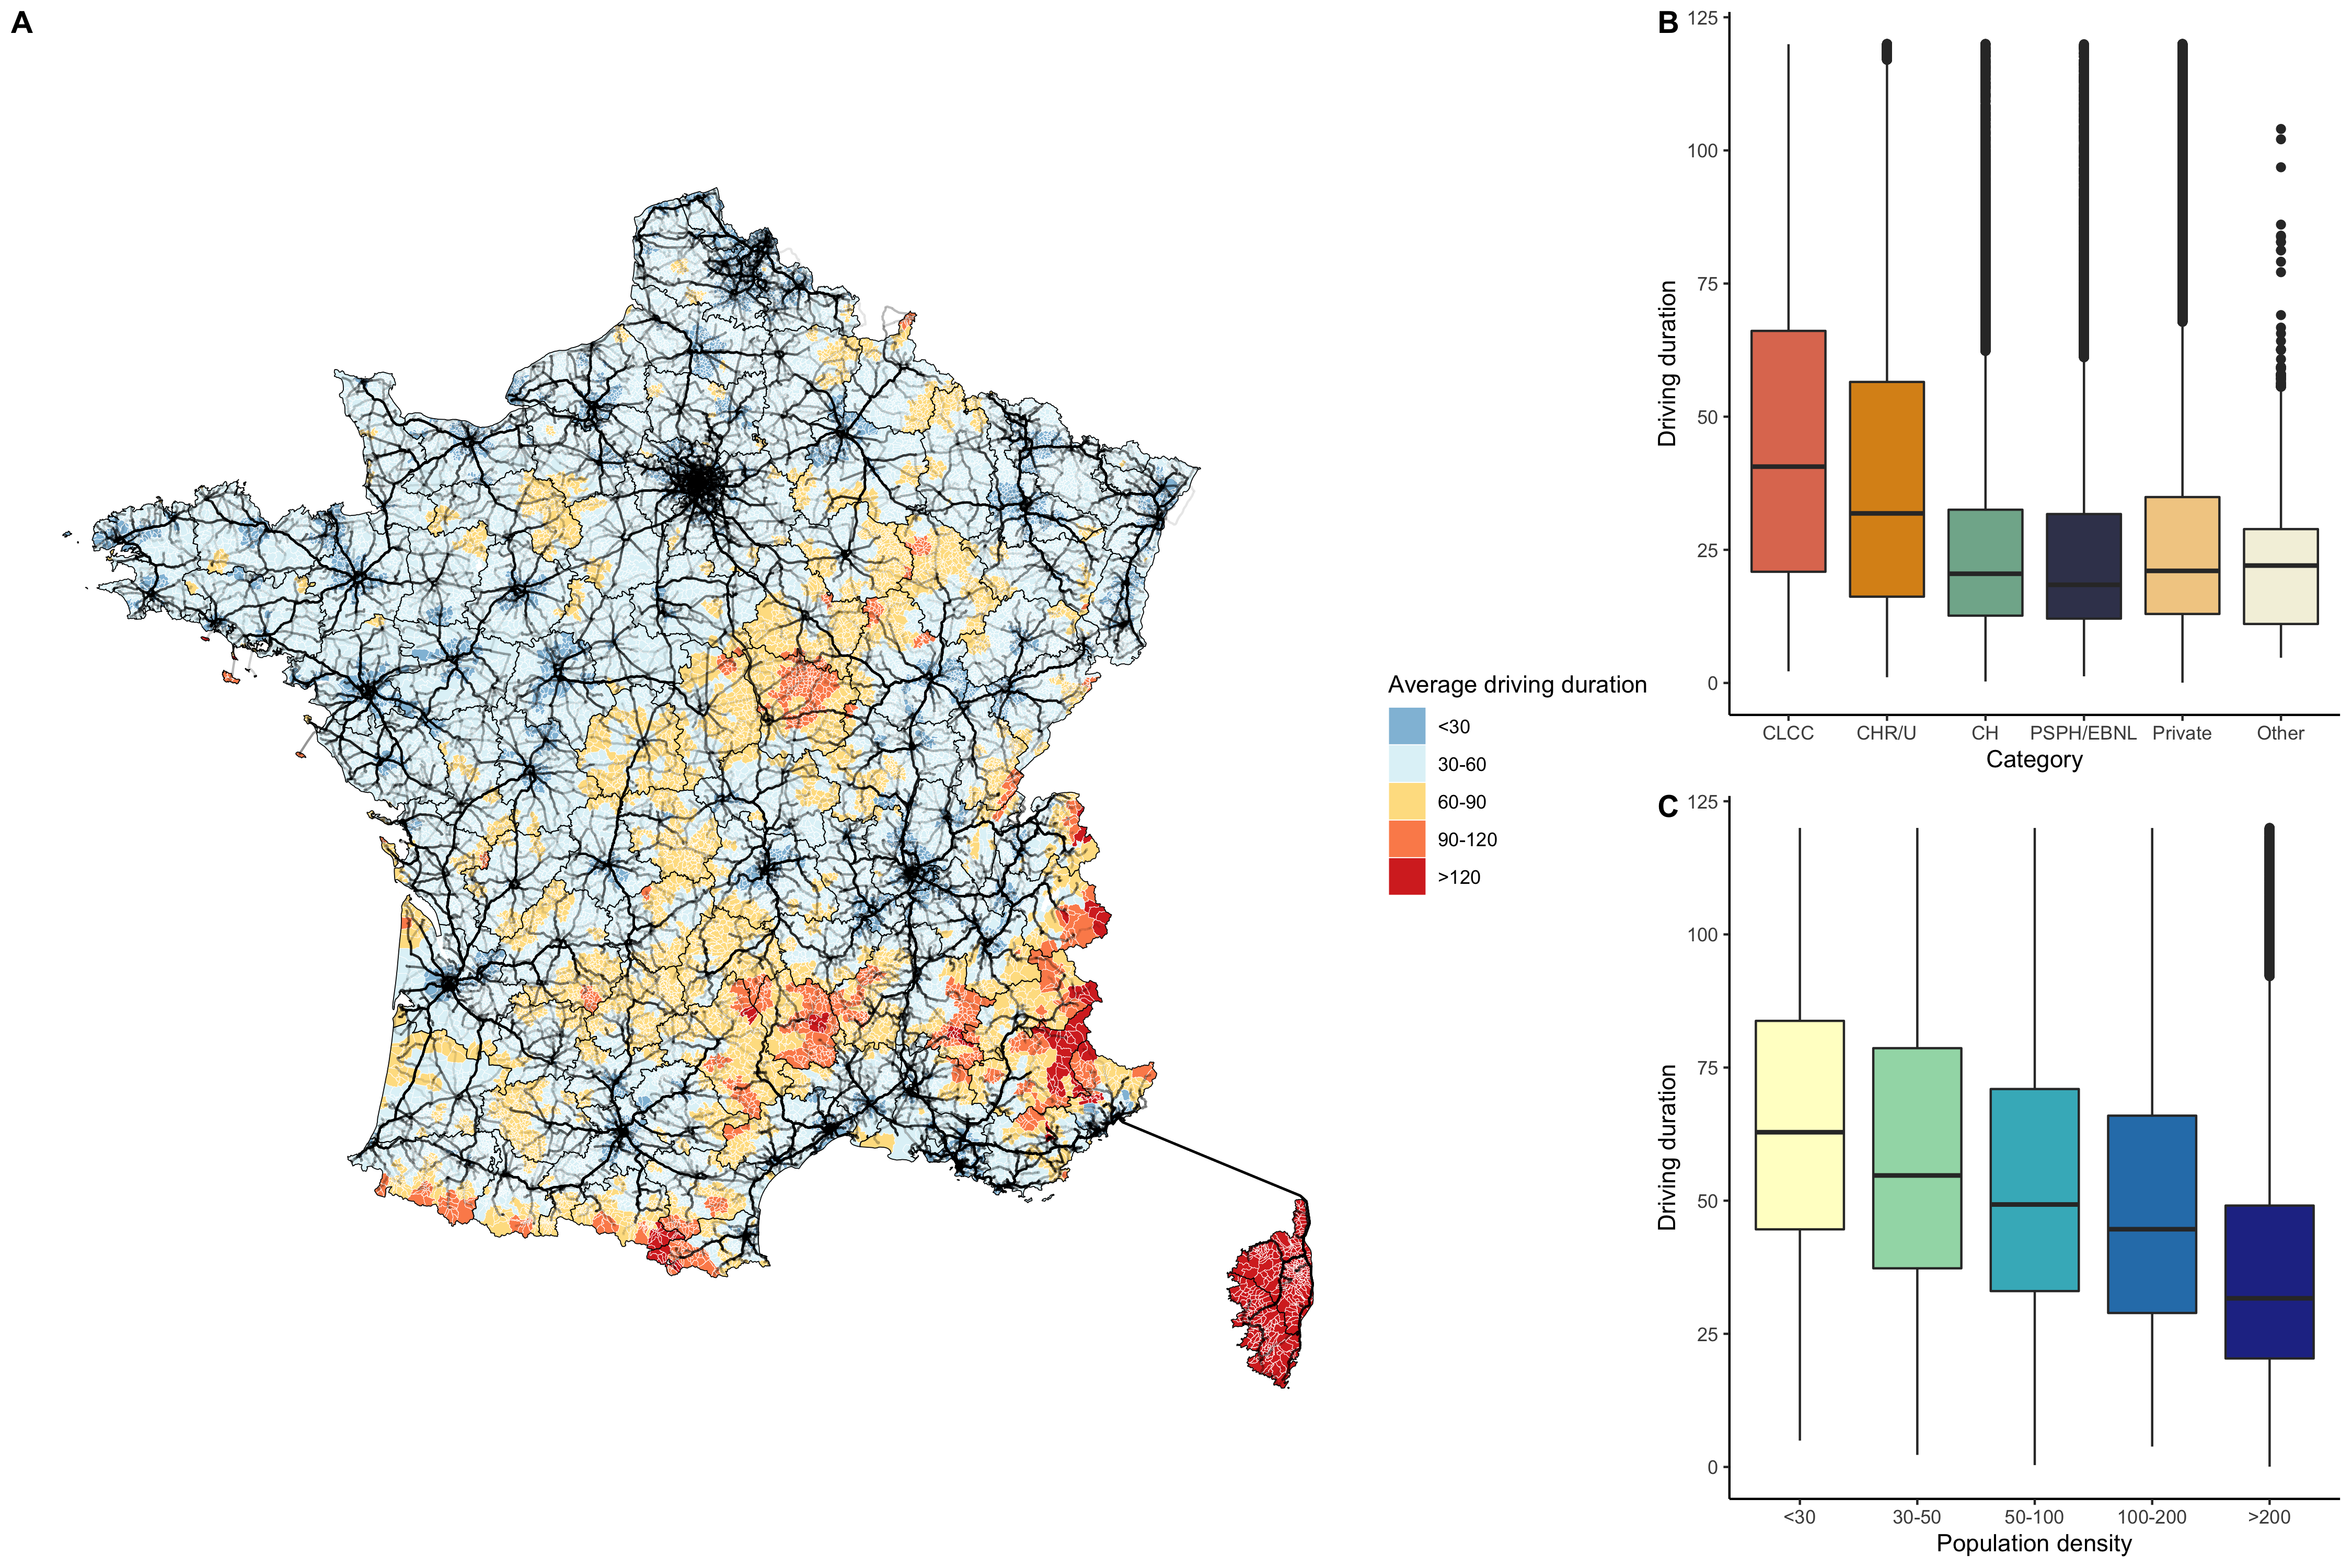
\includegraphics[width=0.9\textwidth]{images/routes/fig1.png}
    \centering
    \caption{
        \textbf{Patients routes in metropolitan France.} GPS routes with more than 5 patients are shown on map (A). Municipalities are colored by the average travel duration for patients with cancer. Patients who visit \ac{clcc} and \ac{chru} hospitals have longer travel durations (B); as well as patients who live in non-dense municipalities (C).
    }
    \label{fig:routes-duration-france}
\end{figure}

\begin{figure}[H]
    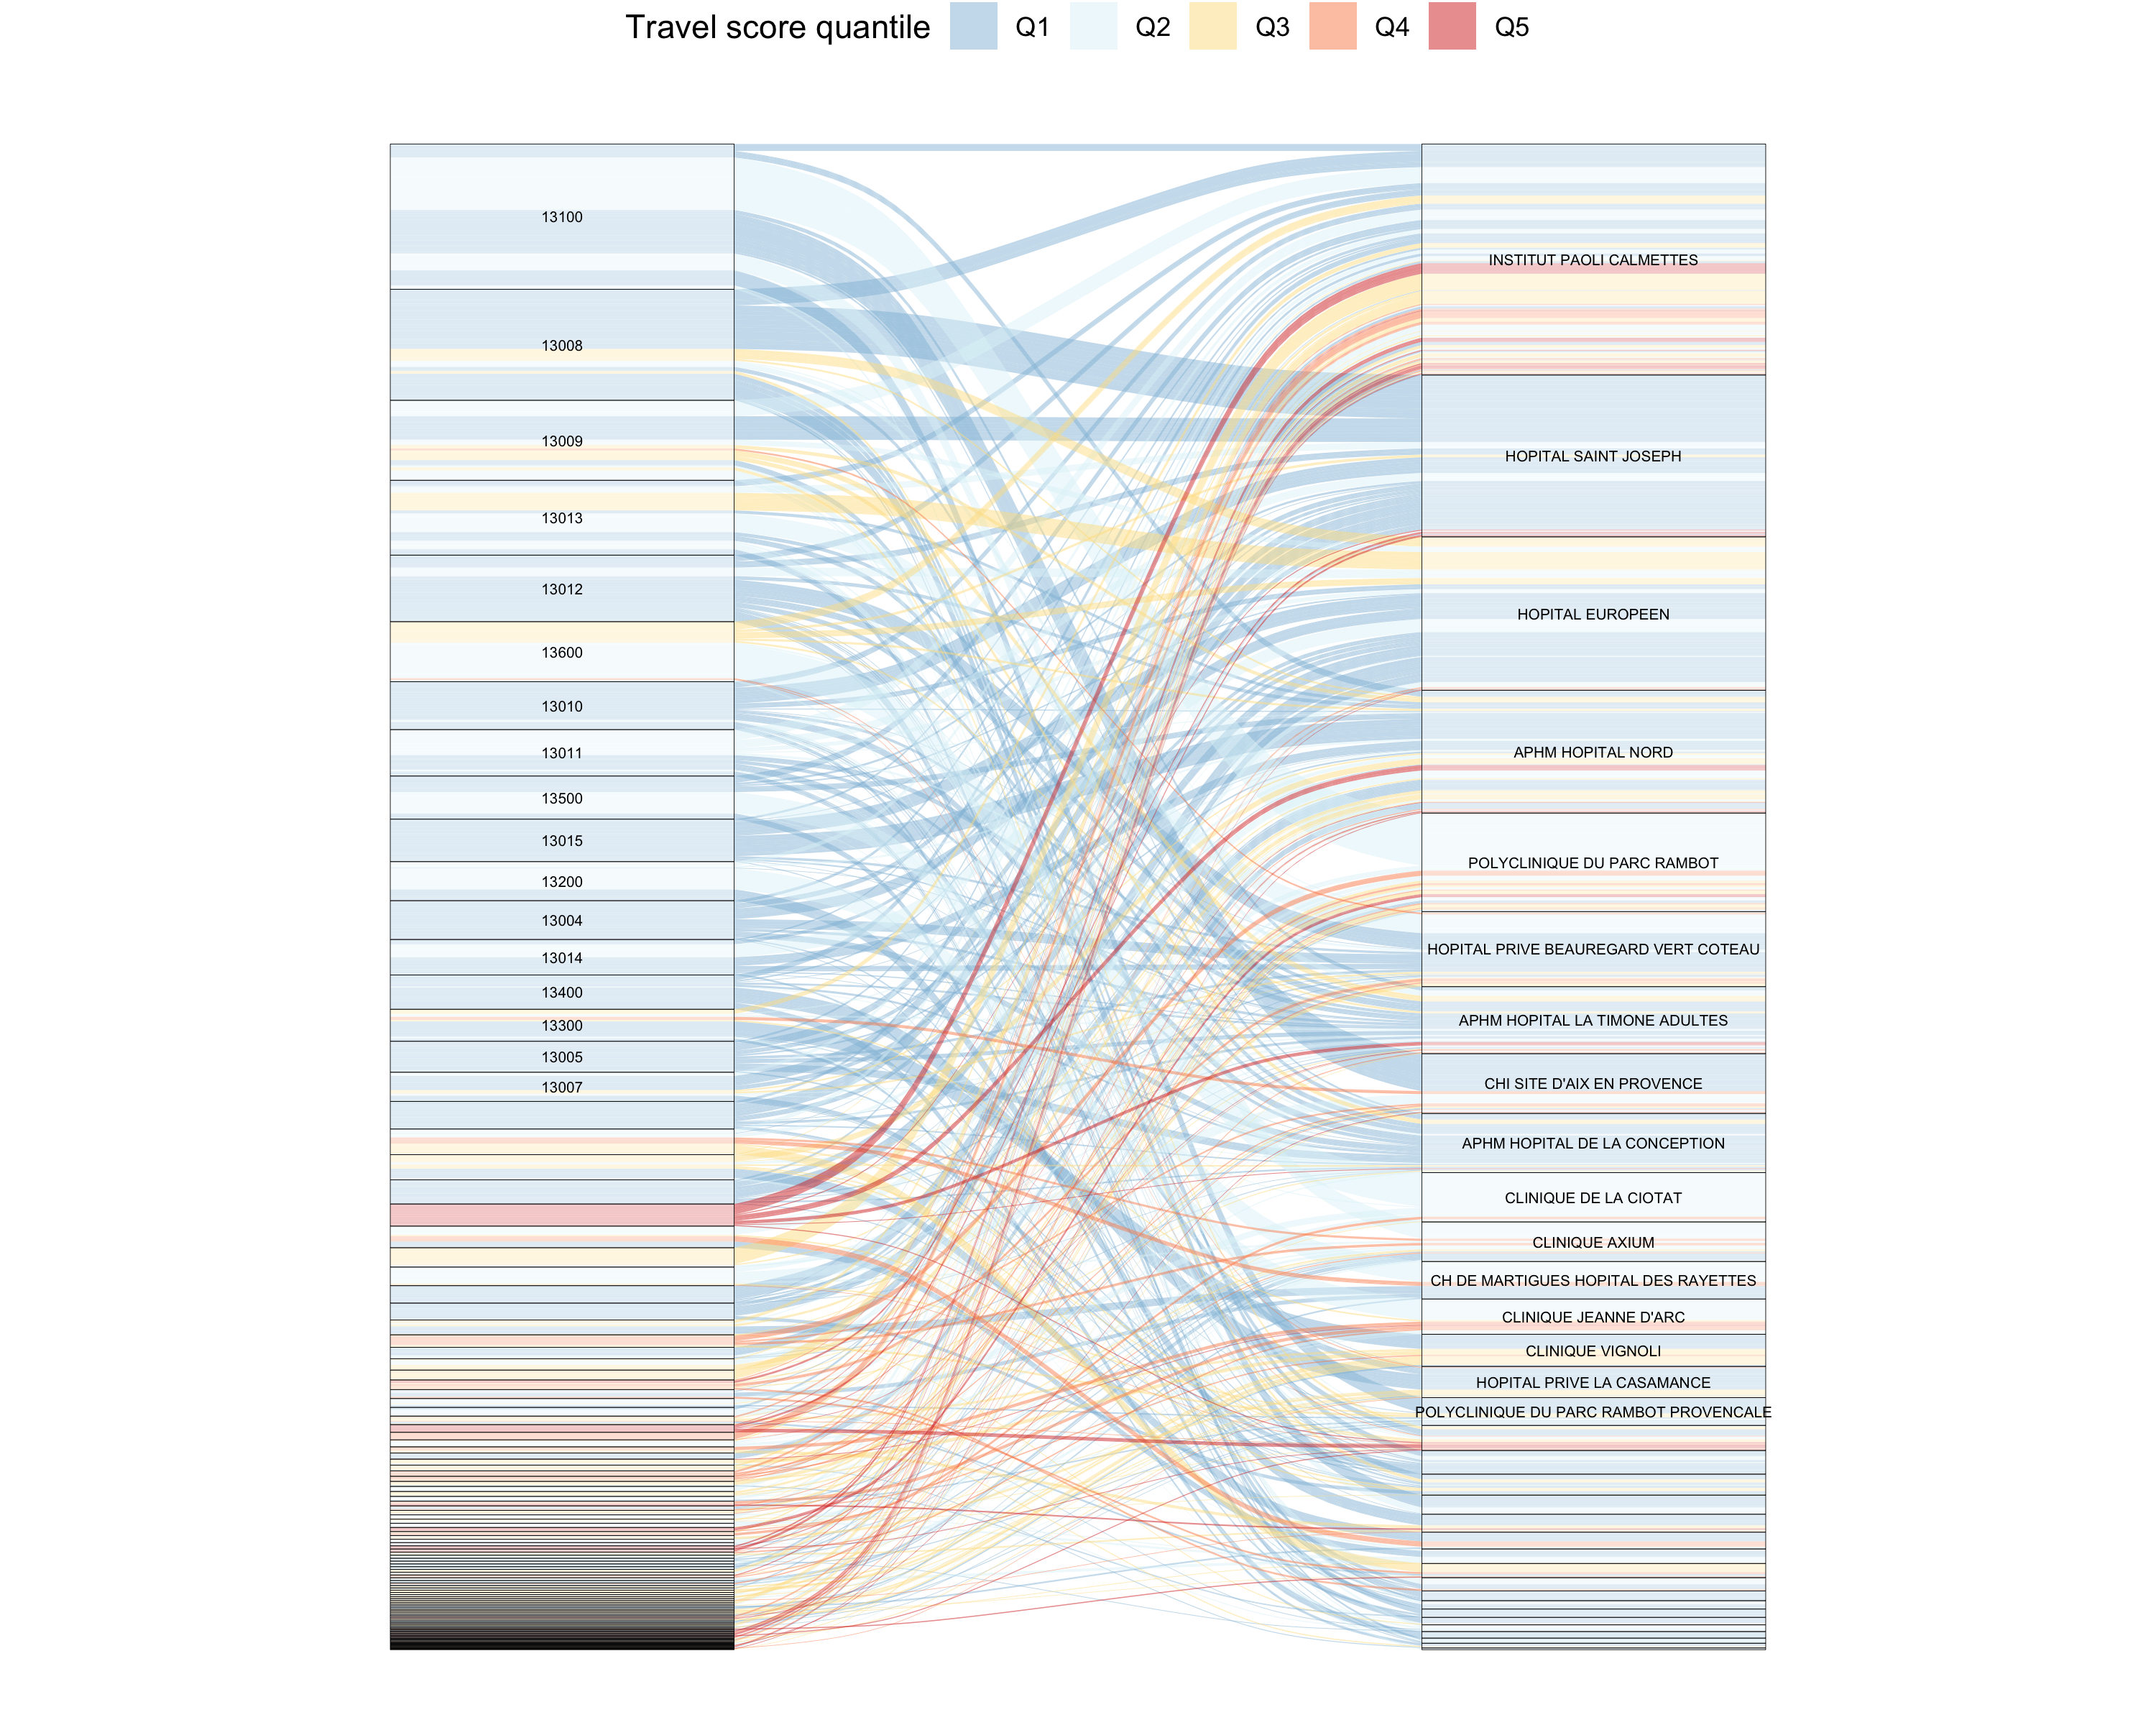
\includegraphics[width=0.9\textwidth]{images/routes/fig6.png}
    \centering
    \caption{
        \textbf{Distribution of patients traveling to care centers located in Bouches-du-Rhone department.} Municipalities are displayed on the right side of the alluvial plot, and care centers on the left side. Municipalities are sized by the number of residing patients. Care centers are sized by the number of treated patients. Flows represent patients travel and are sized by the number of patients traveling from a municipality to a care center. The flows are colored based on the travel score quantile. We can easily identify that the patients living in smaller municipalities are more likely to experience tedious travel. Larger care centers often receive patients from these smaller municipalities.
    }
    \label{fig:routes-alluvial-13}
\end{figure}

\begin{figure}[H]
    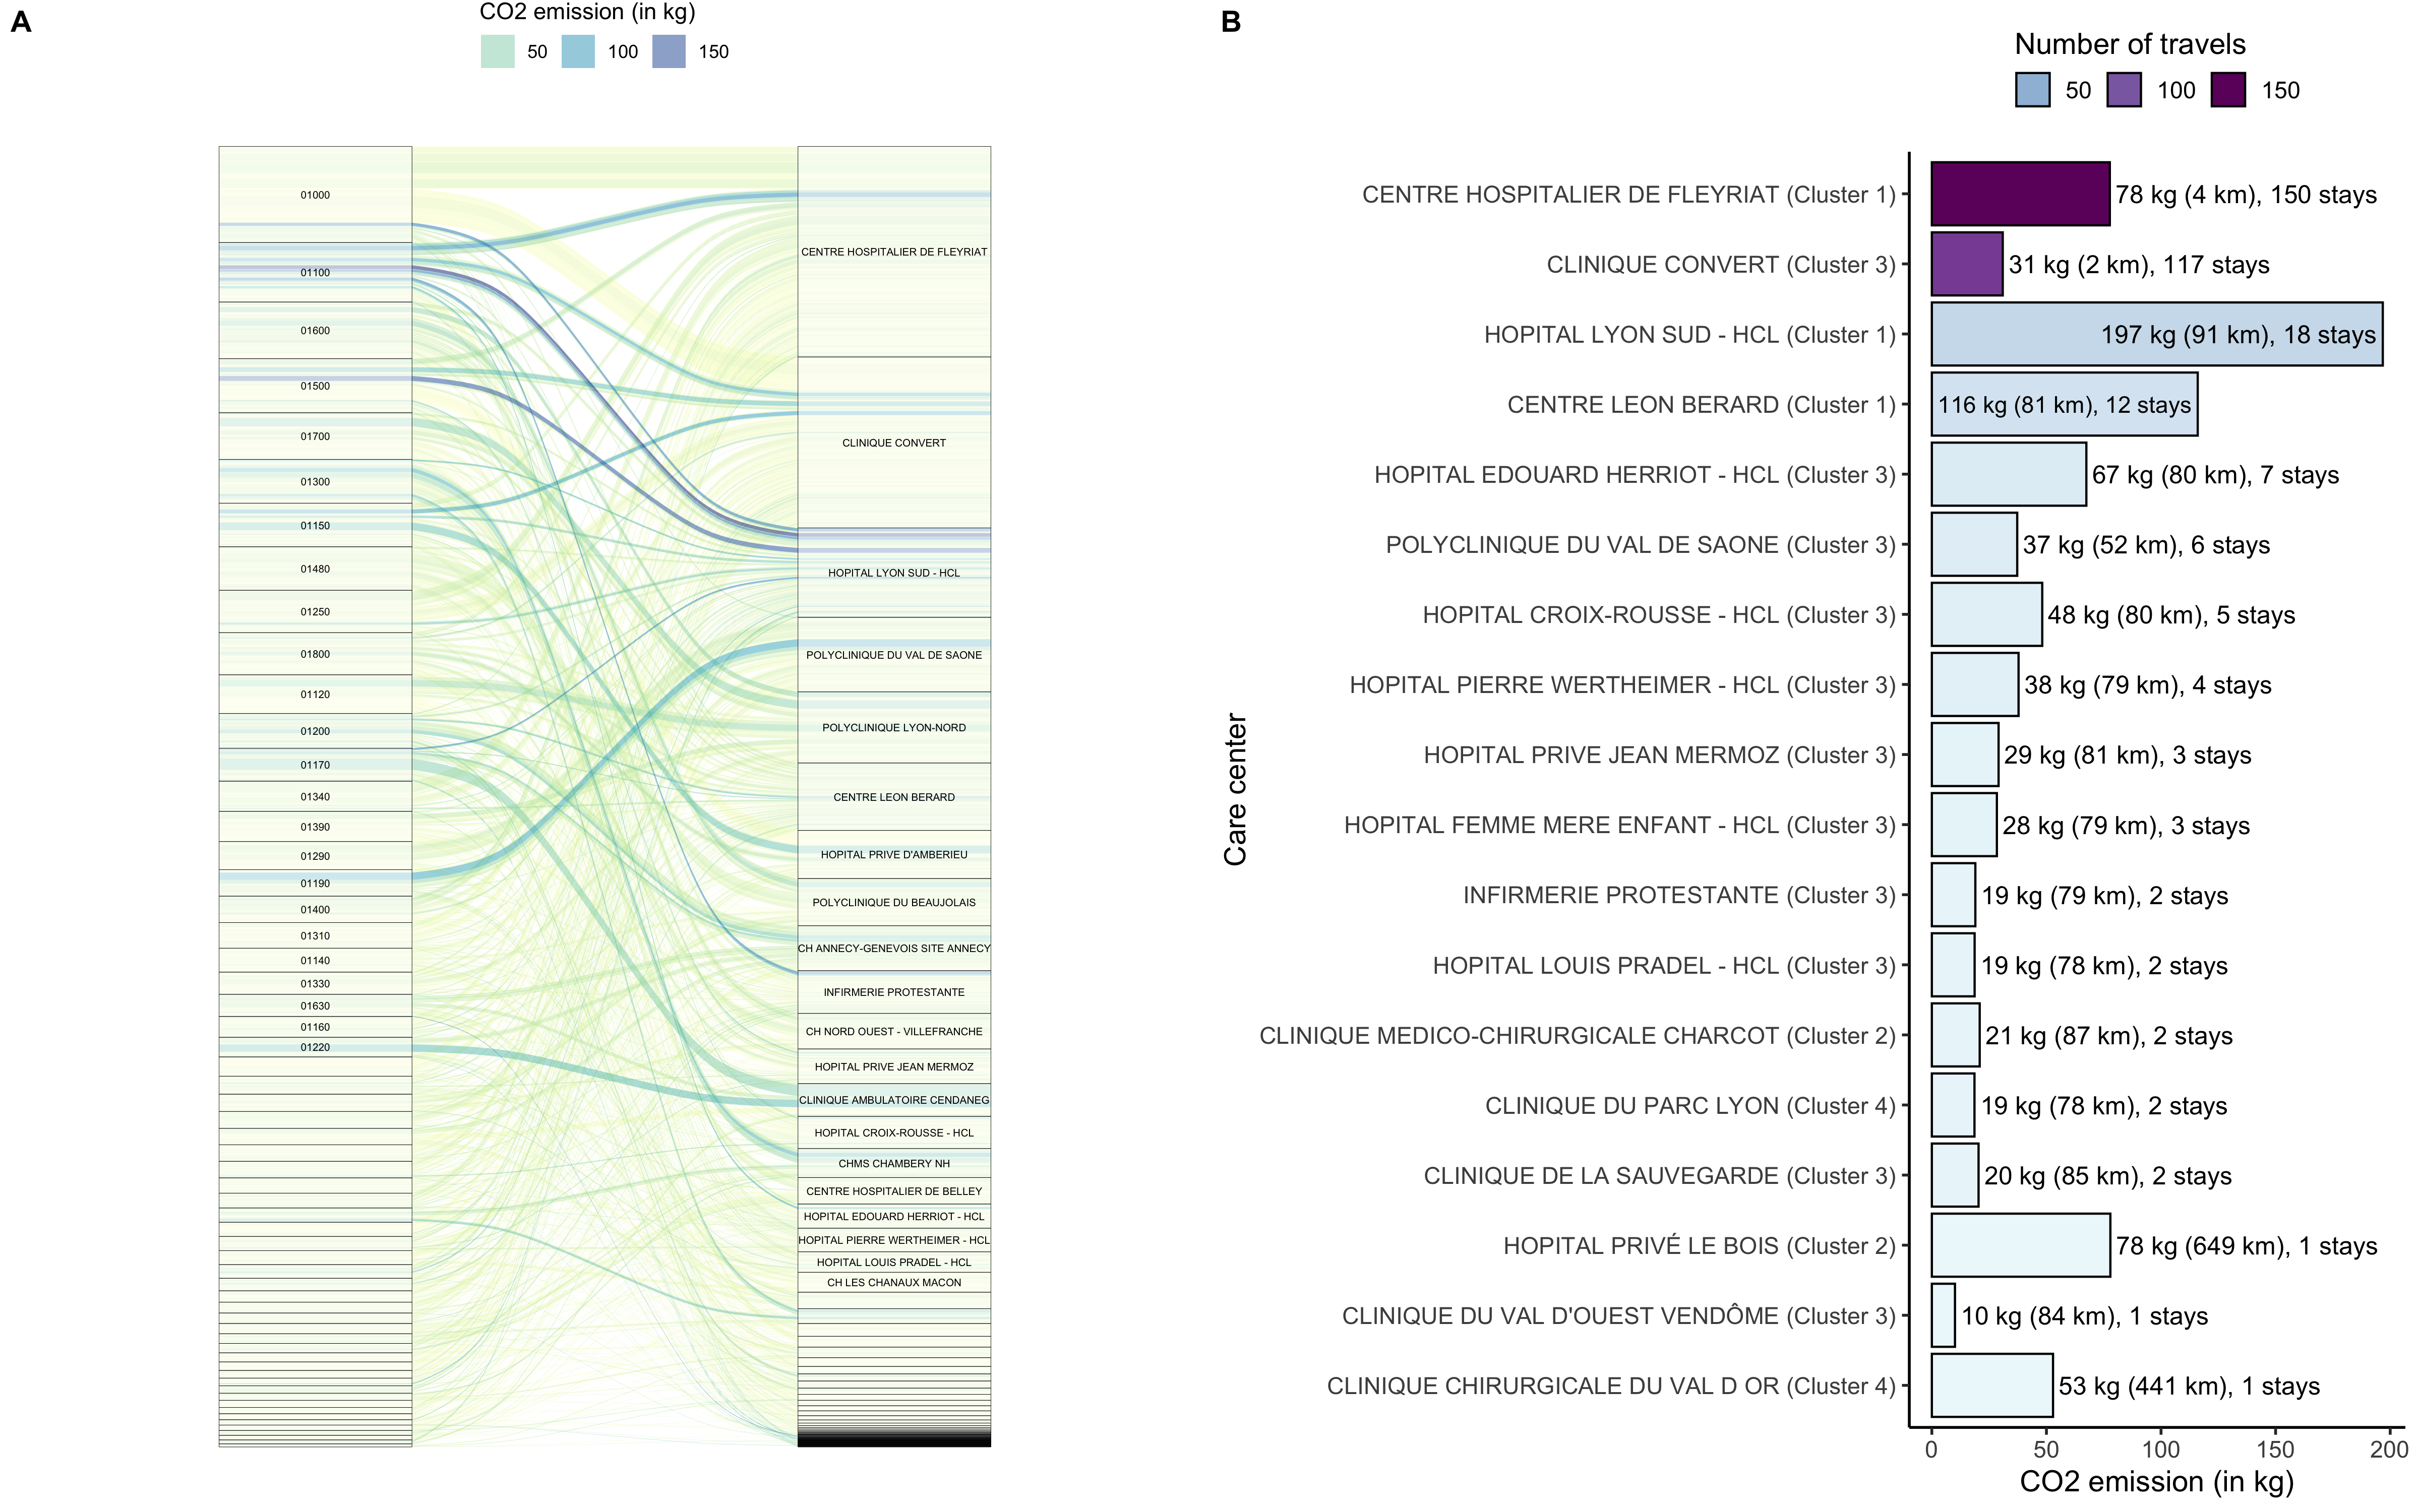
\includegraphics[width=0.9\textwidth]{images/routes/fig8.png}
    \centering
    \caption{
        \textbf{Patients travel, sized by number of travels, and colored by \ac{co2} emission.} We study the patients travel in Bourg-en-Bresse area, a sub-urban and rural area located in Auvergne-Rhone-Alpes region. Plot (A) displays the patients flows from municipalities on the right to care centers on the left. The flows are colored by the resulting \ac{co2} emissions. \ac{co2} emissions are calculated by multiplying the travel distance by the number of travels and the car average consumption. We can see that the higher \ac{co2} emissions are not issued by travels with lots of patients, but instead from travels with fewer patients but much longer drives. This is emphasized on plot (B), showing the \ac{co2} emissions resulting from patients living in Bourg en Bresse area. Indeed, the 42 travels to Hopital Lyon Sud emitted three times as much \ac{co2} than the 253 travels to Centre Hospitalier de Fleyriat.
    }
    \label{fig:routes-co2-01}
\end{figure}
